\documentclass[10pt]{article}

%%notre fichier de configuration perso
\usepackage{rapport_configuration}


\usepackage[smartEllipses]{markdown}
\usepackage{pdfpages}


\title{Rapport de l'unité Projet math/info}
\author{    Thoma Lessage\\
            Pascal Padilla\\
            Raphaël Sellam
    }
\date{\today}



\begin{document}



%%% Titre coloré
\pagecolor{orangeamu!25}
\maketitle\thispagestyle{empty}


%%% Sommaire coloré
\newpage\pagecolor{orangeamu!10}
\tableofcontents


%%% couleur neutre


\newpage
\nopagecolor


\markdownInput{md_wiki/Version_beta.txt.md}


\newpage
\part{Présentation du projet}

\markdownInput{md_wiki/Appel_à_projet.txt.md}
\newpage
\markdownInput{md_wiki/Road_map.txt.md}
\newpage
\markdownInput{md_wiki/Version_alpha.txt.md}


\newpage
\part{Méthodologie de gestion du projet}

\markdownInput{md_wiki/Scrum.txt.md}
\newpage
\markdownInput{md_wiki/Sprint_et_visioconf.txt.md}


\newpage
\part{Outils utilisés}
\markdownInput{md_wiki/Godot.txt.md}
\newpage
\markdownInput{md_wiki/Dépôt_git.txt.md}


\newpage
\part{Documentation et références techniques}
\markdownInput{md_wiki/Générateur_automatique_de_doc.txt.md}
\newpage
\markdownInput{md_wiki/Duel_button.md}
\newpage
\markdownInput{md_wiki/Game_generator.md}
\newpage
\markdownInput{md_wiki/Round_buttons.md}
\newpage
\markdownInput{md_wiki/Score_manager.md}
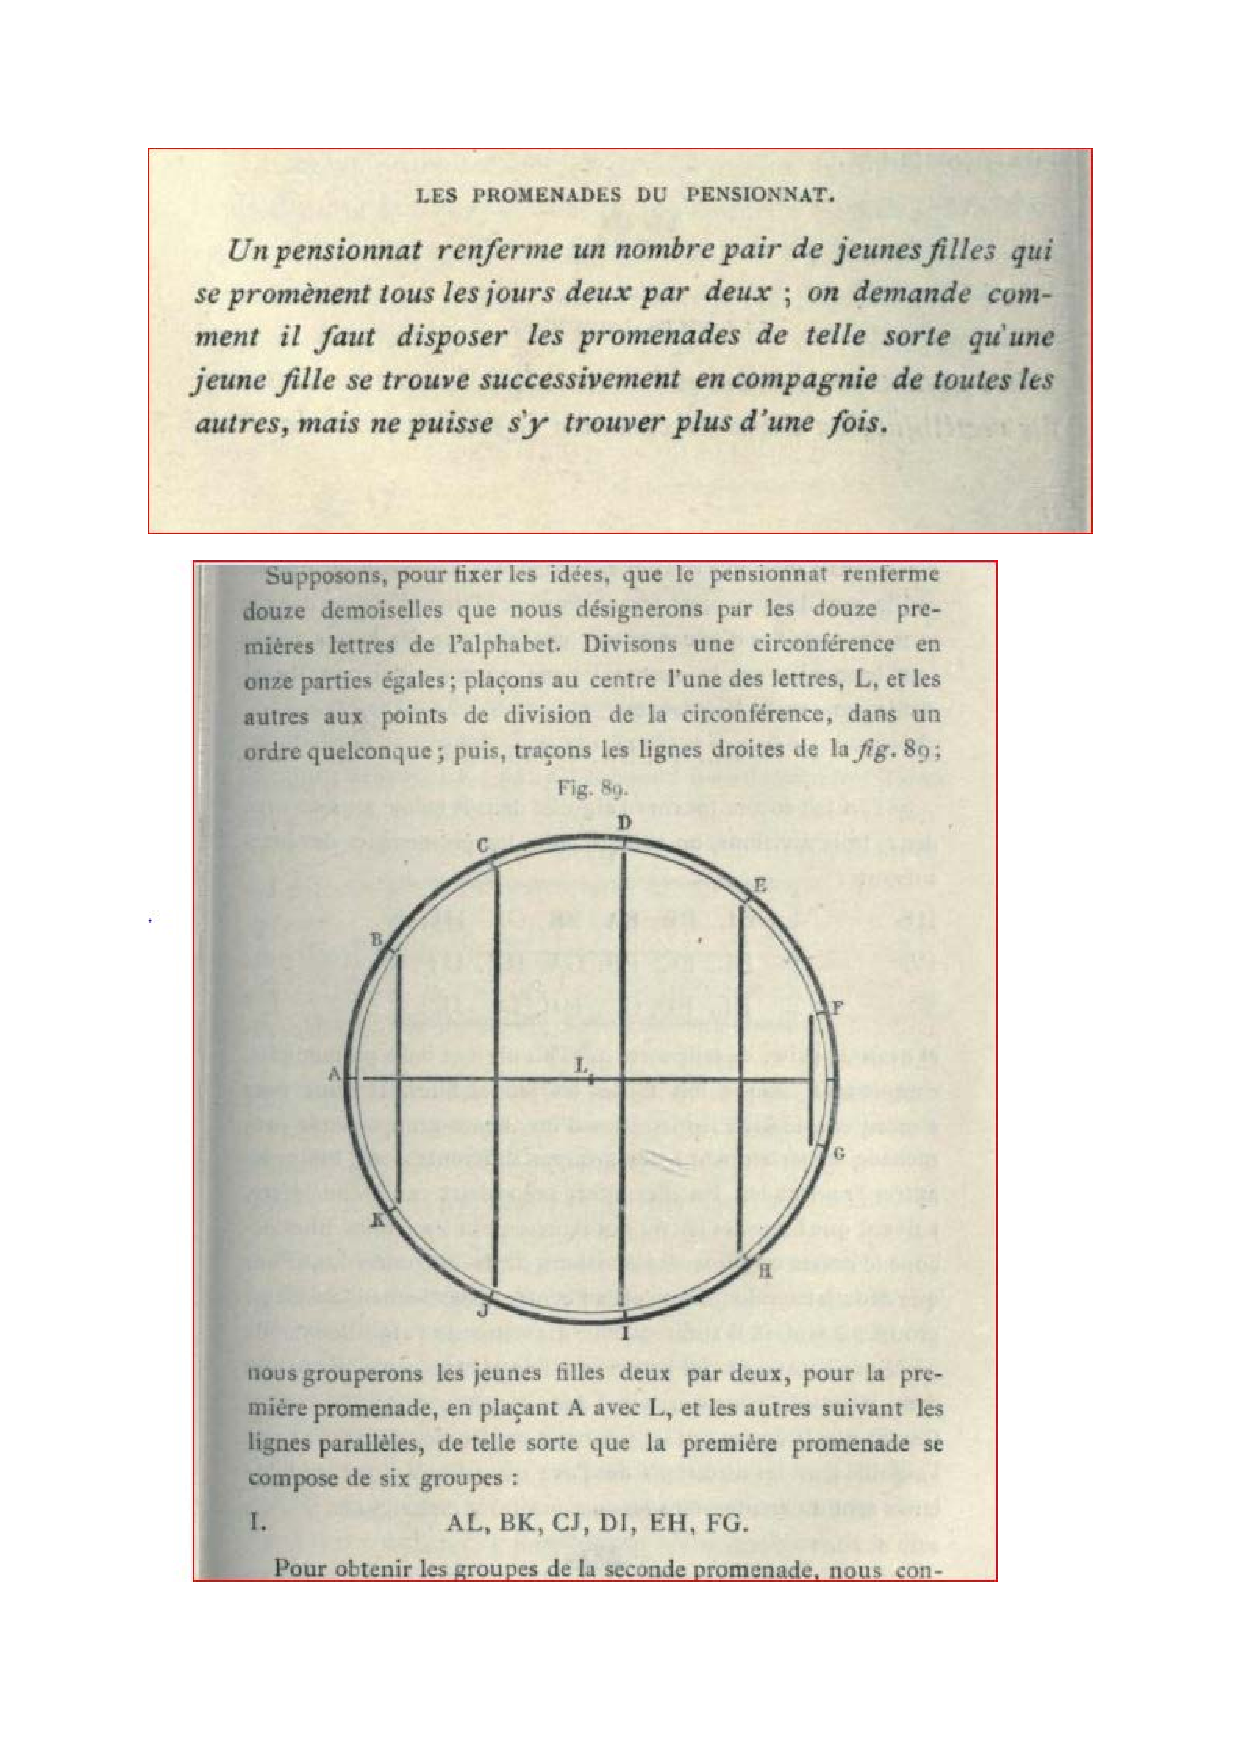
\includepdf[scale=.8, page=1, pagecommand=\section{Une approche mathématique}]{md_wiki/Projet_Tournois.pdf}
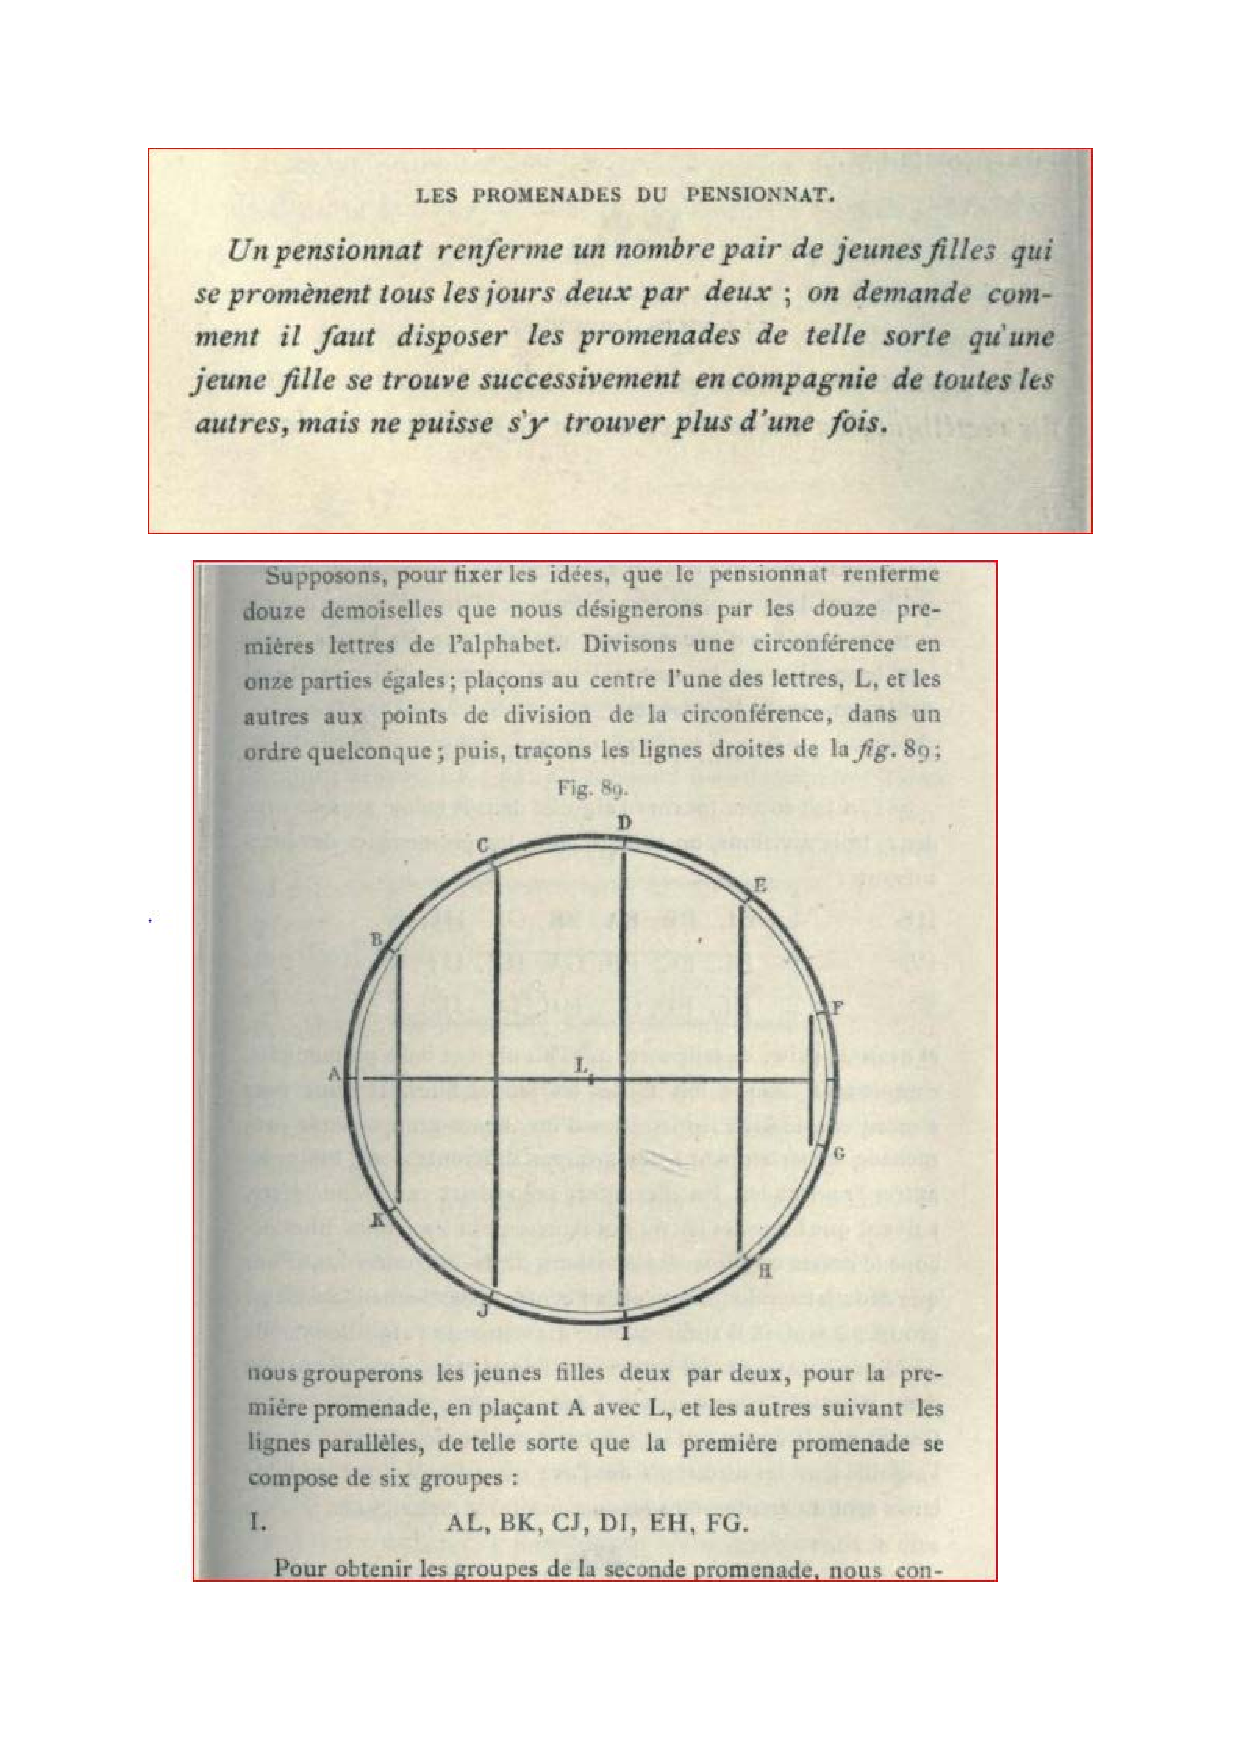
\includepdf[scale=.9, page=2-4]{md_wiki/Projet_Tournois.pdf}
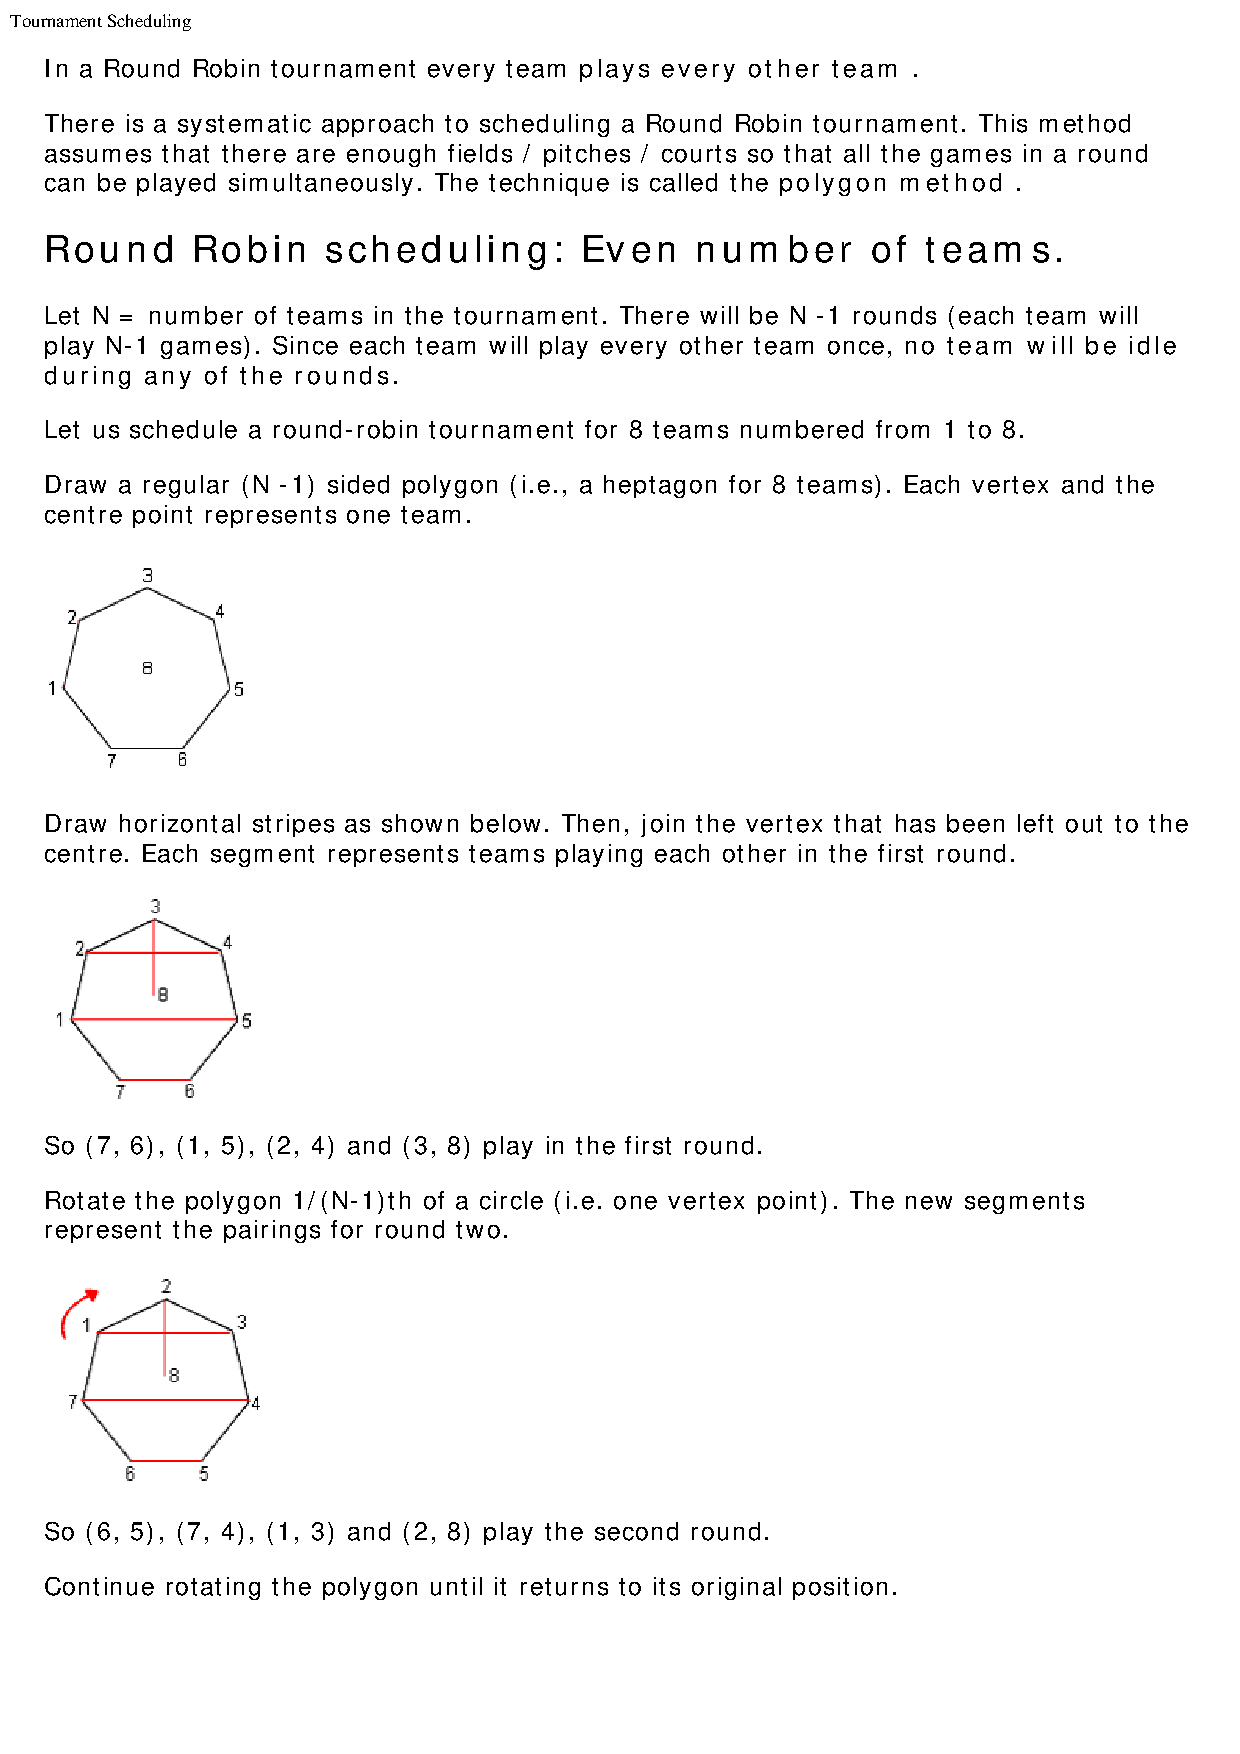
\includepdf[scale=.9, page=2-4]{md_wiki/Projet_Tournois_Bis.pdf}



\end{document}